\documentclass[12pt]{article}
\usepackage{fullpage}
\usepackage{amsmath}
\usepackage{amssymb}
\newtheorem{proof}{PROOF}
\usepackage{algorithm}
\usepackage{algpseudocode}
\usepackage{graphicx}
\graphicspath{ {images/} }

\title{Homework 3}
\author{Young Won Kim (yk41) and Minh Pham (mnp7)}
\date{Spring 2017}
 
\begin{document}
\maketitle

\noindent \textbf{1 MAP and MLE parameter estimation} \\

\noindent \textbf{Part 1. Using MLE}\\
\\
$D = \{x^{(i)} \mid 1 \leq i \leq m; x \in \{0,1\}\} $
\\
\\
Probability mass function of each $x^{(i)}$:\\

\indent $f(x^{(i)}; \theta) = \theta ^{x^{(i)}} (1-\theta)^{(1-x^{(i)}}$ \\
\\
Likelihood function:\\

\indent $L(\theta) = \prod_{i=1}^m \theta^{x^{(i)}} (1-\theta)^{(1-x^{(i)})}$
\\ 
\\
Maximum likelihood function:\\

\indent $L(\theta) = \theta ^{\sum_{i=1}^m x^{(i)}} (1-\theta)^{(m - \sum_{i=1}^m x^{(i)})}$\\

\indent $\theta = argmax_{\theta} L(\theta) = argmax_{\theta} log(L(\theta))$\\

\indent $\theta = argmax_{\theta} \sum_{i=1}^m x^{(i)} log(\theta) + (m - \sum_{i=1}^m x^{(i)}) log (1-\theta)$\\
\\
\indent $\frac{\partial log(L(\theta))}{\partial \theta} = \frac{\sum_{i=1}^m x^{(i)}} {\theta} - \frac{(m-\sum_{i=1}^m x^{(i)})}{1-\theta} \equiv 0$\\
\\
\indent $\sum_{i=1}^m x^{(i)} (1-\theta) - (m-\sum_{i=1}^m x^{(i)})\theta = 0$\\

$\sum_{i=1}^m x^{(i)} - m\theta = 0$\\
\\
\indent $\widehat{\theta} = \frac{\sum_{i=1}^m x^{(i)}} {m}$
\pagebreak

\noindent \textbf{Part 2. Using MAP}\\
\\
$P(\theta) = \theta^{(a-1)} (1-\theta)^{(b-1)}$\\
\\
$\widehat{\theta} = argmax_\theta P(D \mid \theta) P(\theta) = argmax_\theta \prod_{i=1}^m \theta^{x^{(i)}} (1-\theta)^{(1-x^{(i)})} \theta^{(a-1)} (1-\theta)^{(b-1)}$\\
\\
$\widehat{\theta} = argmax_\theta \sum_{i=1}^m x^{(i)}log(\theta) + (m - \sum_{i=1}^m x^{(i)}) log(1-\theta) + log(\theta) (a-1) + (b-1) log(1-\theta)$\\
\\
$\frac{\partial L(\theta)}{\partial \theta} = \frac {\sum_{i=1}^m x^{(i)}} {\theta} - \frac {(m-\sum_{i=1}^m x^{(i)})} {1-\theta} + \frac{a-1}{\theta} - \frac{b-1}{1-\theta} \equiv 0$
\\
\\
$0 = \sum_{i=1}^m x^{(i)} (1-\theta) - \theta (m-\sum_{i=1}^m x^{(i)}) + (a-1)(1-\theta) - \theta(b-1)$\\
\\
$0 = \sum_{i=1}^m x^{(i)} + \theta (-m -a -b +2 ) -1 + a$
\\
\\
With a = b = 1, we have:\\
\\
$\theta = \frac {\sum_{i=1}^m x^{(i)}} {m}$
\\
\\
\noindent \textbf{2 Logistic regression and Gaussian Naive Bayes} \\
\\
\noindent \textbf{Part 1 Logistic regression}
\\
\\
$P(y = 1 \mid x; \theta) = g(\theta^Tx) ; \theta \in \mathbb{R} ^{d + 1}$\\
\\
$P(y = 0 \mid x; \theta) = 1- g(\theta^Tx)$\\
\\
where $g(\theta^Tx) = \frac {1}{1 + e ^{-\theta^{T}x}} $
\\
\\
\noindent \textbf{Part 2 Gaussian Naive Bayes}
\\
\\
$P(y = 1 \mid x) = \frac{P(x \mid y = 1) P(y = 1)} {P(x)} = \frac {P(x \mid y = 1) P (y = 1) }{P(x \mid y = 1) P(y =1) + P (x \mid y = 0) P (y = 0)}$
\\
\\
$P(y = 1 \mid x) = \frac {1} {1 + \frac{P(y = 0) P(x \mid y = 0)}{P(y = 1)P(x \mid y = 1)}}$
\\
\\
$P(y = 1 \mid x) = \frac {1} {1 + exp(ln \frac {P(y = 0) P(x \mid y = 0)}{P(y = 1)P(x \mid y = 1)})}$
\\
\\
$P(y = 1 \mid x) = \frac {1} {1 + exp(ln \frac {P(y = 0}{P(y = 1)} + ln \frac{P(x \mid y = 0)}{P(x \mid y = 1)})}$
\\
\\
We have:
\\
\\
$\frac {P(y = 0)}{P(y = 1)} =  \frac {1 - \phi}{\phi}$
\\
\\
And:
\\
\\
$ln \frac{P(x \mid y = 0)}{P(x \mid y = 1)} = \sum_{j=1}^d (ln \frac {P(x_j \mid y = 0)} {P(x_j \mid y = 1)}$
\\ 
\\
$ln \frac{P(x \mid y = 0)}{P(x \mid y = 1)} =\sum_{j=1}^d ln \frac {\frac{1}{\sqrt{2\pi \sigma ^2}} exp (\frac {-(x_j + \mu_{j 0})^2}{2\sigma_j^2})}{\frac{1}{\sqrt{2\pi \sigma ^2}} exp (\frac {-(x_j + \mu_{j 1})^2}{2\sigma_j^2})} $
\\
\\
$ln \frac{P(x \mid y = 0)}{P(x \mid y = 1)} =\sum_{j=1}^d ln exp (\frac {(x_j - \mu_{j 1})^2 - (x_j - \mu_{j 0})^2} {2\sigma_j^2}) = \sum_{j=1}^d (\frac{\mu_{j 0} - \mu_{j 1}}{\sigma_j^2} x_j + \frac{\mu_{j 1} ^2 - \mu_{j 0} ^2} {\sigma_j^2})$
\\
\\
Therefore,
\\
\\
$P(y = 1 \mid x) = \frac{1}{1 + exp (w_0 + \sum_{j=1}^d w_j x_j)}$,
\\
\\
in which,
\\
$w_0 = ln \frac {1-\phi}{\phi} + \sum_{j=1}^d \frac{\mu_{j 1} ^2 - \mu_{j 0} ^2} {\sigma_j^2}$
\\
$w_j = \frac{\mu_{j 0} - \mu_{j 1}}{\sigma_j^2}$
\\
\\
$P(y = 0 \mid x) = 1 - P(y = 1\mid x) = \frac{exp(w_0 + \sum_{j=1}^d w_j x_j)} {1 + exp (w_0 + \sum_{j=1}^d w_j x_j)}$
\\
\\
\noindent \textbf{Part 3 Uniform Class Priors}
\\
\\
Since class 1 and class 0 are equally likely, we have:
\\
\\
$\frac {P(y = 0)}{P(y = 1)} =  \frac {1 - \phi}{\phi} = 1$
\\
\\
Therefore,
\\
\\
$P(y = 1 \mid x) = \frac{1} {1 + exp \sum_{j=1}^d (\frac{\mu_{j 1}^2 - \mu_{j 0}^2}{2\sigma_j^2} + \frac{\mu_{j 0} - \mu_{j 1}}{\sigma_j ^2} x_j)}$
\\
\\
We call:
\\
\\
$\theta_0 = \frac{\mu_{j 1}^2 - \mu_{j 0}^2}{2\sigma_j^2}$
\\
\\
$\theta_j = \frac{\mu_{j 0} - \mu_{j 1}}{\sigma_j ^2} $
\\
\\
Therefore,
\\
\\
$P(y = 1 \mid x) = \frac{1}{1+exp(\theta_0 +  \sum_{j=1}^d (\theta_j x_j))} = \frac{1}{1 + exp (\theta^T x)} \equiv P(y = 1 \mid x) $ for logistic regression\\
\\
\\
\\
\noindent \textbf{3 Reject Option In Classifiers}
\\
\\
\noindent \textbf{Part 1 Minimum Risk}
\\
\\
Risk for choosing an action i is:\\
\\
\indent $R (\alpha_i \mid x) = \sum_{j = 1}^C L(\alpha = i, y = j) P(y = 1 \mid x)$ for $i = 1 , ..., C$ \\
\\
\indent $R (\alpha_i \mid x) = \sum_{j = 1, j \neq i}^C \lambda_s P(y = j \mid x) = \lambda_s (1 - P(y = i \mid x))$\\
\\
Risk for a rejection is:\\
\\
\indent $R (\alpha_{C+ 1} \mid x) = \lambda_r$ \\
\\
Minimal risk that is obtained when we decide $y = j$ is:\\
\\
\indent $\lambda_r \leq \lambda_s (1 - P(y = i \mid x)) $ with $ i = 1, ..., C$\\
\\
Therefore, \\
\\
\indent $P(y = i \mid x) \leq 1 - \frac {\lambda_r}{\lambda_s} $ with $i =  1 , ... ,  C$\\
\\
In addition, in an intuitive sense, we also have to choose the most probable class, which means $P(y = j \mid x) \leq P(y = k \mid x)$ for all k
\\ 
\\
\noindent \textbf{Part 2 The loss ratio between reject and misclassification increases from 0 to 1}
\\
\\
As $\frac {\lambda_1} {\lambda_2}$ increases from 0 to 1, the loss of rejection increases. When $\frac {\lambda_1} {\lambda_2}= 1$, the loss of rejection is larger than the loss of misclassification, and we shouldn't choose the rejection option.\\
\\
\noindent \textbf{4 One$\_$vs$\_$all logistic regression and softmax regression}\\
\\
- As $\theta$ is initially generated randomly, there is no preference for the class y belongs to, and therefore probability is equal for each classes, $\frac{1}{10}$. If we sum up accross $m$ examples and divide by $m$, the loss results to $-log(0.1)$.\\
\\
- Naive loss: 2.365103 computed in 26.325576s\\
- Vectorized loss: 2.365103 computed in 0.607100s
\\
- Loss difference: 0.000000
\\
- Gradient difference: 0.000000\\
\\
- The best value for learning rate and regularization strength are:
lr=1.000000e-06, reg=1.000000e+05. This resulted in validation accuracy of 41.6$\%$. \\
\\
- The best softmax classier on the test set resulted in overall accuracy of  40.8$\%$. \\
\\
- Comparing OVA vs SOFTMAX on CIFAR-10: OVA yielded lower recall, precision, and accuracy compared to Softmax. Sofmax works better on datasets where the features aren't obviously related to specific classes, which makes it a better classifier for CIFAR-10. Empirical data also supports this, as Softmax performed better than OVA in terms of recall, precision, and accuracy.
\\

\begin{figure}[!tpb]
	\centerline{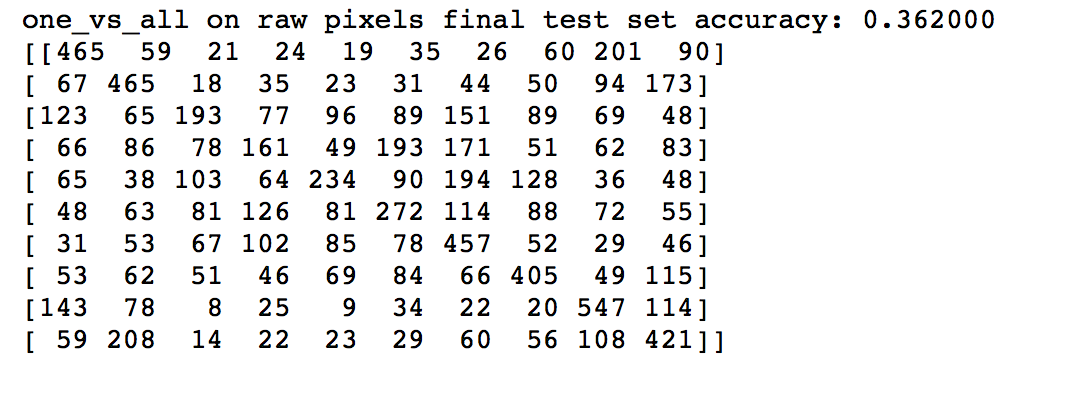
\includegraphics[width=80mm]{OVA_conf}}
	\caption{\label{fig1}
		Confusion matrix of OVA }
\end{figure}

\begin{figure}[!tpb]
	\centerline{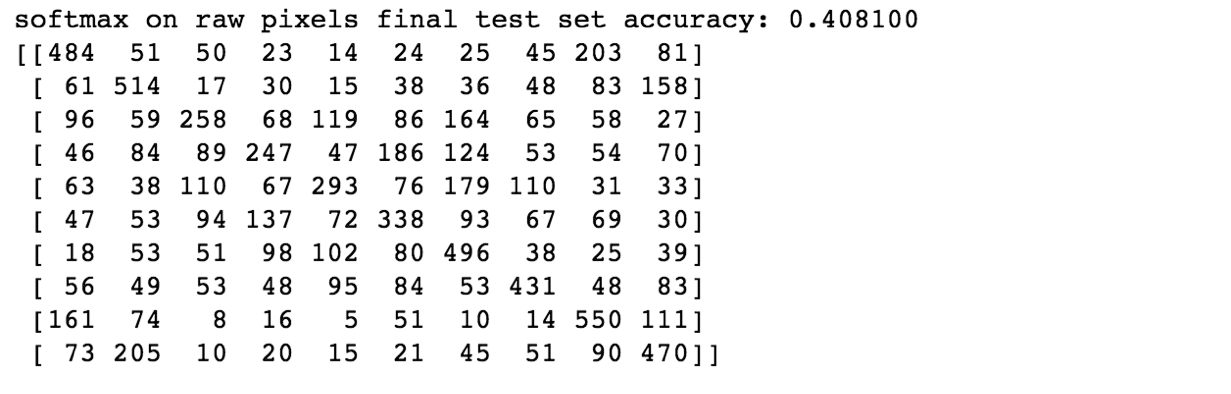
\includegraphics[width=80mm]{SOFTMAX_conf}}
	\caption{\label{fig2}
		Confusion matrix of SOFTMAX}
\end{figure}

\begin{figure}[!tpb]
	\centerline{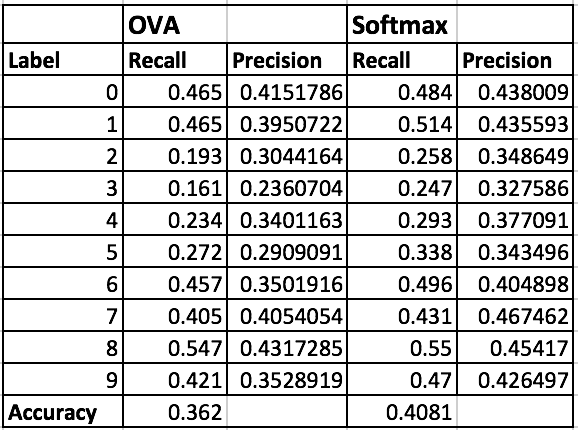
\includegraphics[width=80mm]{precision_recall.png}}
	\caption{\label{fig3}
		Comparison between OVA and SOFTMAX - precision, recall, accuracy}
\end{figure}

\begin{figure}[!tpb]
	\centerline{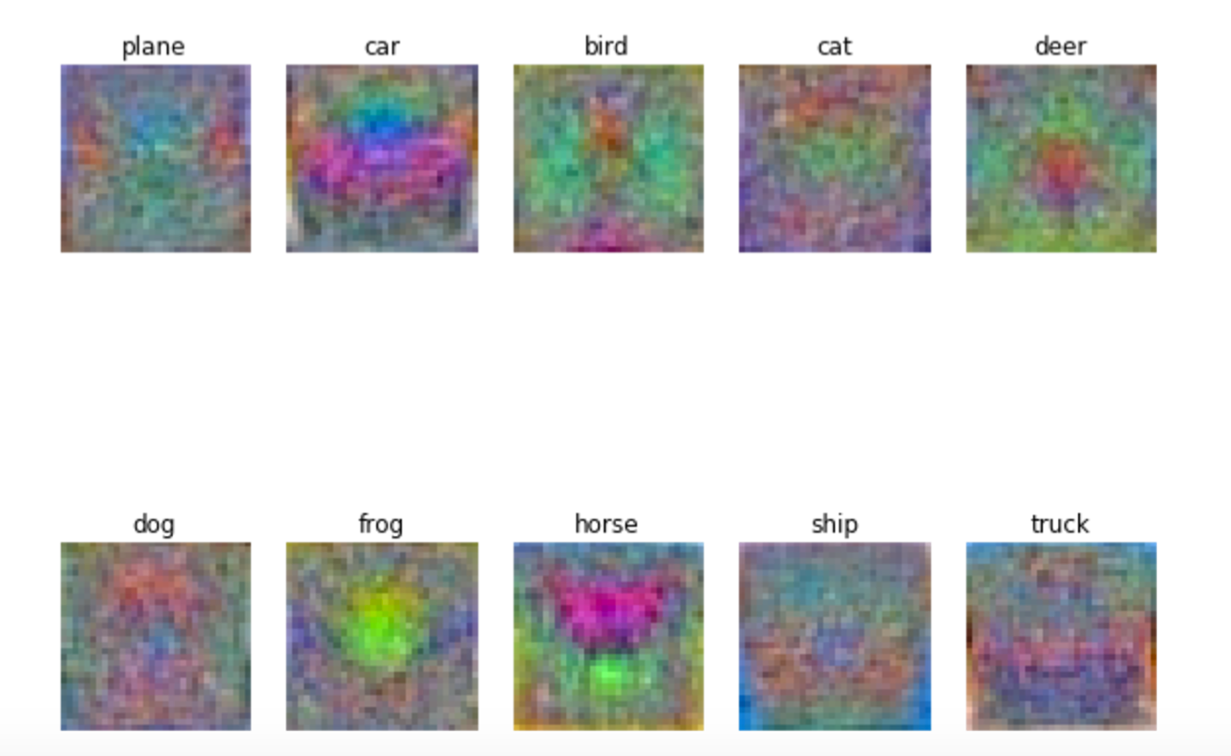
\includegraphics[width=80mm]{CIFAR-10.png}}
	\caption{\label{fig4}
		Visualization of the learned parameter matrix}
\end{figure}

\noindent- The visualized coefficients corresponds to the importance of each pixel in determining the class. Bluer color represent higher correlation between the class and the pixel.\\

\pagebreak
\noindent \textbf{Extra Credit}
\begin{figure}[!tpb]
	\centerline{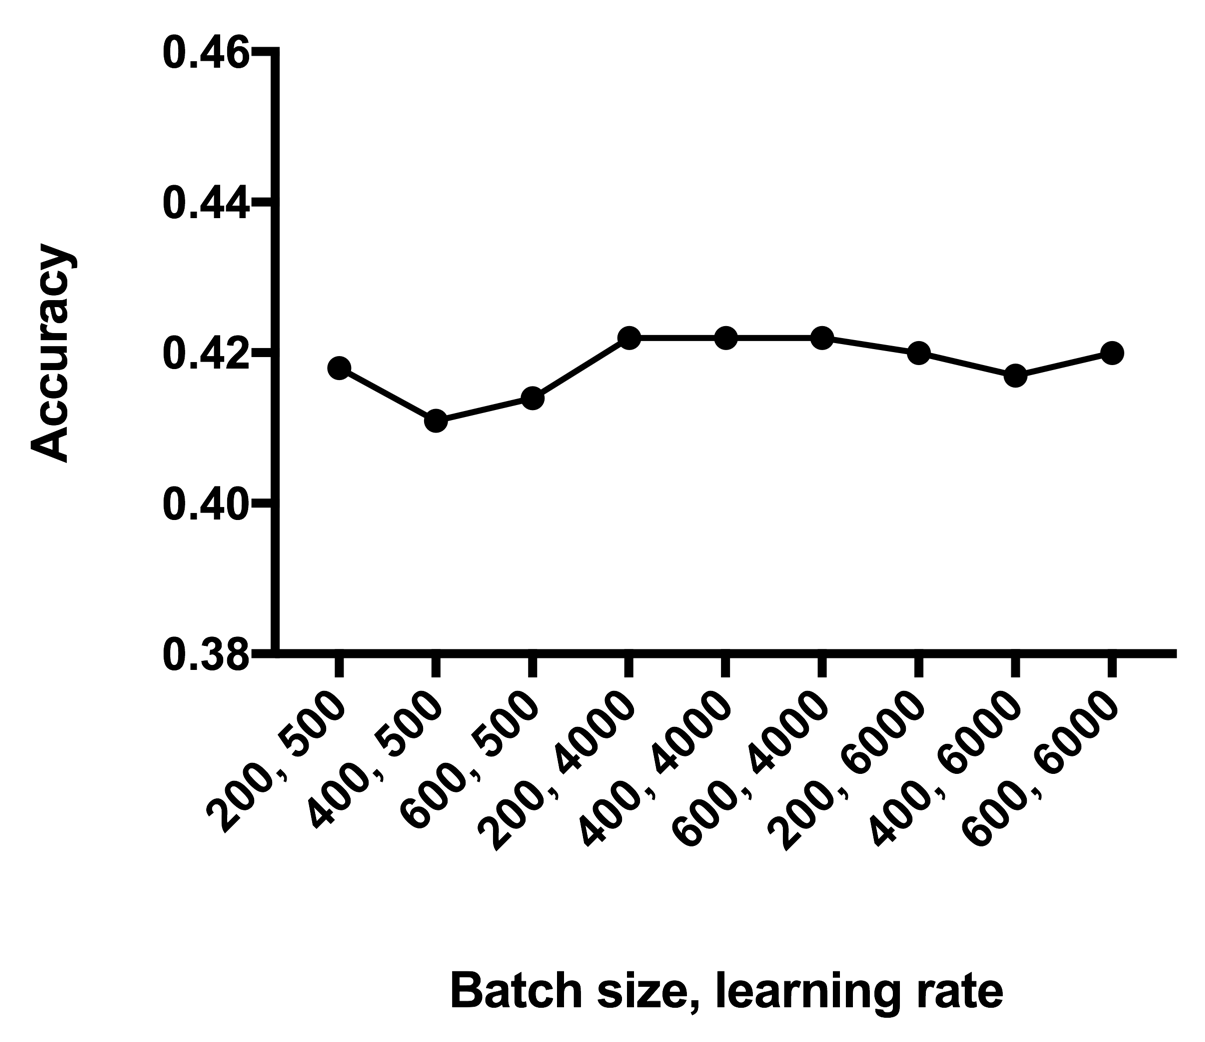
\includegraphics[width=80mm]{ExtraCredit.png}}
	\caption{\label{fig5}
		Other hyperparameters and their accuracies}
\end{figure}

\noindent Based on runs with different hyperparameters, we found that higher batch size and number of iterations tend to result in higher accuracy. However, increasing the batch size and number of iterations too much also leads to overfitting. The number of iterations that yielded the best accuracy was 4000, regardless of the batch size, highest accuracy being 0.422 (Fig.5).\\
\\
\noindent Selected runs and their hyperparameters:\\
200 batch size, 500 iterations, lr 5.0e-07, reg 1.0e+05: train accuracy of 0.395, val accuracy of 0.418\\
400 batch size, 500 iterations, lr 1.0e-06, reg 1.0e+05: train accuracy of 0.403, val accuracy of 0.411\\
600 batch size, 500 iterations, lr 1.0e-06, reg 5.0e+05: train accuracy of 0.405, val accuracy of 0.414\\
200 batch size, 4000 iterations, lr 5.0e-07, reg 1.0e+05: train accuracy of 0.403, val accuracy of 0.422\\
400 batch size, 4000 iterations, lr 1.0e-06, reg 5.0e+04: train accuracy of 0.412, val accuracy of 0.422\\
600 batch size, 4000 iterations, lr 1.0e-06, reg 1.0e+05: train accuracy of 0.409, val accuracy of 0.422\\
200 batch size, 6000 iterations, lr 5.0e-07, reg 1.0e+05: train accuracy of 0.406, val accuracy of 0.420\\
400 batch size, 6000 iterations, lr 5.0e-07, reg 5.0e+04: train accuracy of 0.413, val accuracy of 0.417\\
600 batch size, 6000 iterations, lr 5.0e-07, reg 5.0e+04: train accuracy of 0.412, val accuracy of 0.420\\

\end{document}
